\textbf{Based on the theorems of chapter 8 of Approximation Theory and Approximation Practice by Trefethen, what can you say about the convergence as $n\rightarrow\infty$ of the Chebyshev interpolants to the following functions? Which is the case that converges much faster than the theorems predict? Can you speculate why?}
\newline

The convergence, predicted by \textsc{Theorem 8.2}, is 
\begin{align*}
\|f-p_n\|\leq\frac{4M\rho^{-n}}{\rho-1},
\end{align*}
with 
\begin{align*}
\rho = \alpha+\sqrt{\alpha^2-1}~~~~\text{(real singularity at $x=\pm\alpha$)},
\end{align*}
or
\begin{align*}
\rho = \beta+\sqrt{\beta^2+1}~~~~\text{(imaginary singularity at $x=\pm i\beta$)}.
\end{align*}

Applying this to the following functions we obtain:
\begin{enumerate}[label=\alph*)]
\item $f(x) = \tan(x)$. This function has a real singularity at $x=\pm \pi/2$. Hence, 
\begin{align*}
\rho = \frac{\pi}{2}+\sqrt{\frac{\pi^2}{4}-1},
\end{align*}
and we have obtained the rate of convergence showed in the next figure.
\begin{figure}[H]
\centering
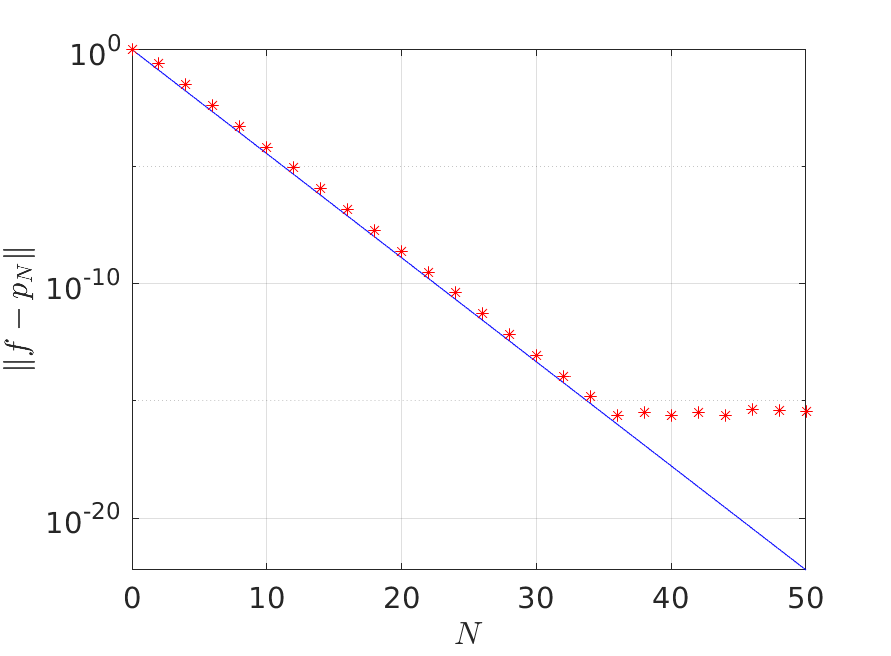
\includegraphics[scale=0.75]{tan(x).png}\caption{Convergence as $n\rightarrow\infty$ of the Chebyshev interpolant to $f(x)=\tan(x)$.}
\end{figure}


\item $f(x) = \tanh(x)$. This function has a imaginary singularity at $x=\pm i\pi/2$. Hence, 
\begin{align*}
\rho = \frac{\pi}{2}+\sqrt{\frac{\pi^2}{4}+1},
\end{align*}
and we have obtained the rate of convergence showed in the next figure.
\begin{figure}[H]
\centering
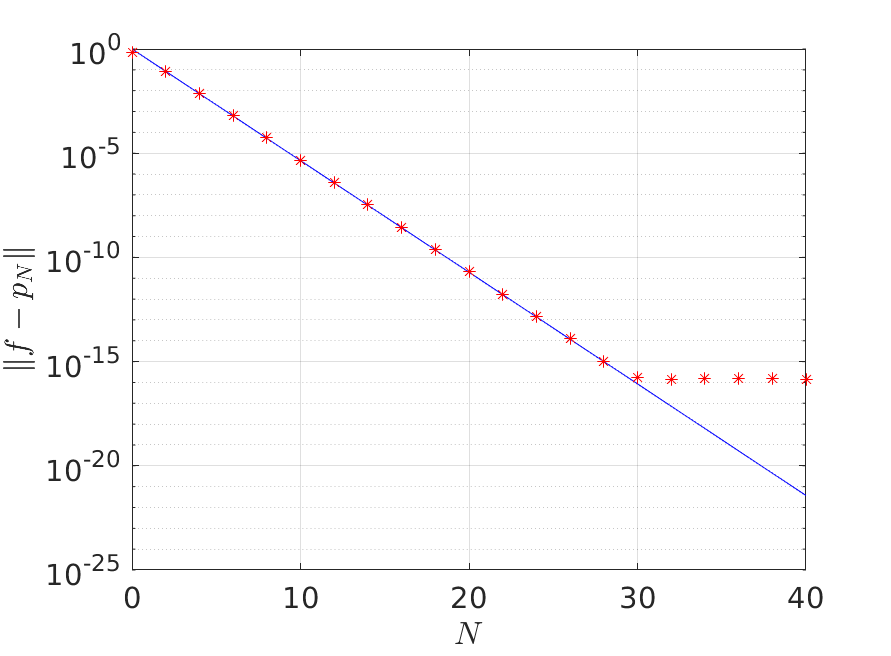
\includegraphics[scale=0.75]{tanh(x).png}\caption{Convergence as $n\rightarrow\infty$ of the Chebyshev interpolant to $f(x)=\tanh(x)$.}
\end{figure}


\item $f(x) = \frac{\log(\frac{x+3}{4})}{x-1}$. This function has a real singularity at $x=-3$. Hence, 
\begin{align*}
\rho = 3+\sqrt{8},
\end{align*}
and we have obtained the rate of convergence showed in the next figure.
\begin{figure}[H]
\centering
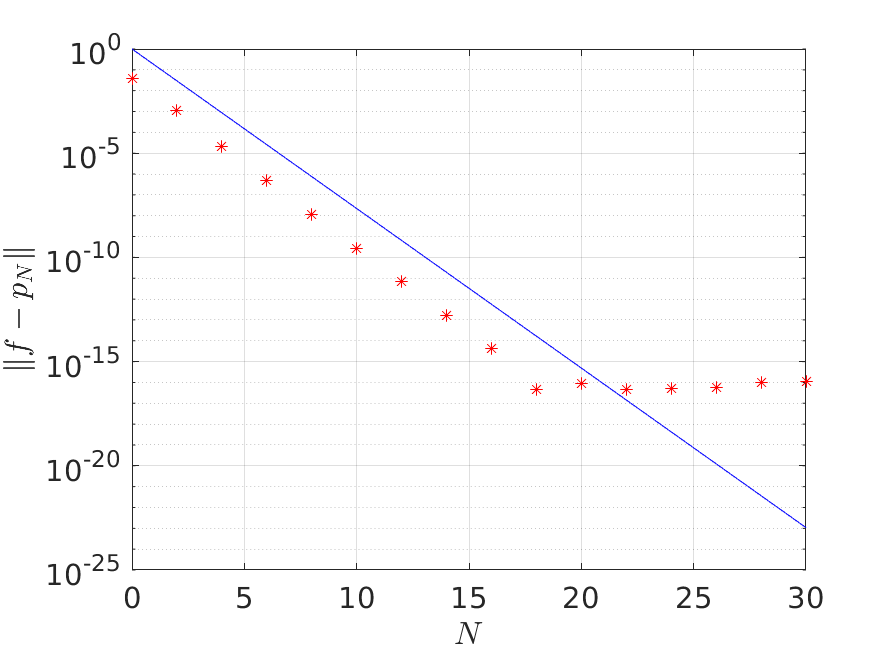
\includegraphics[scale=0.75]{log1.png}\caption{Convergence as $n\rightarrow\infty$ of the Chebyshev interpolant to $f(x)= \frac{\log(\frac{x+3}{4})}{x-1}$.}
\end{figure}

\item $f(x) = \int_{-1}^{x}\cos(t^2)dt$. This function is entire, analytic at all finite points of the complex plane. Hence its convergence is much faster as is shown in the following figure.
\begin{figure}[H]
\centering
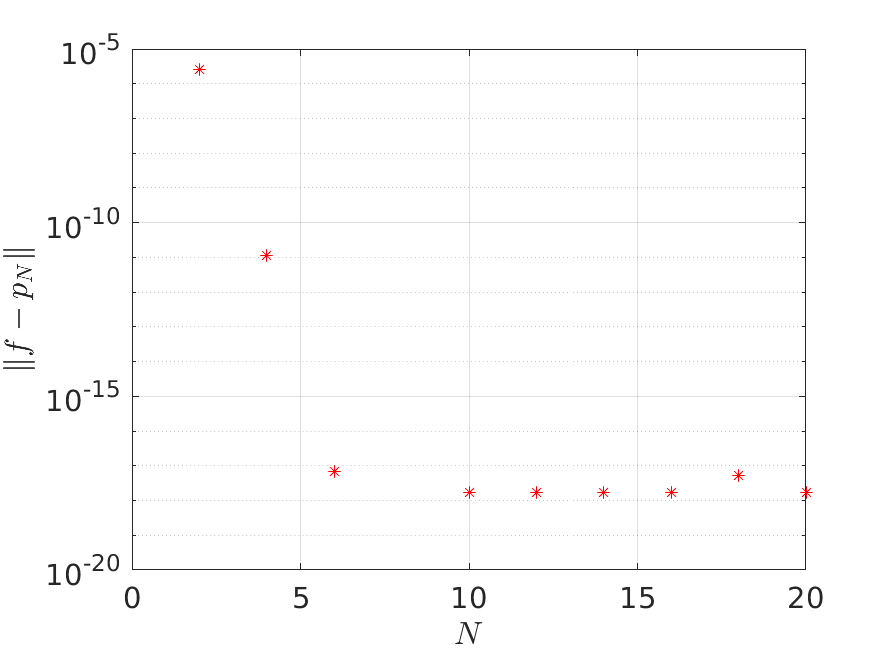
\includegraphics[scale=0.75]{integral.png}\caption{Convergence as $n\rightarrow\infty$ of the Chebyshev interpolant to $f(x)= \frac{\log(\frac{x+3}{4})}{x-1}$.}
\end{figure}



\item $f(x) = \tan(\tan(x))$. This function has a real singularity at $x=\pm \arctan(\pi/2)=\pm k$. Hence, 
\begin{align*}
\rho = k+\sqrt{k^2-1},
\end{align*}
and we have obtained the rate of convergence showed in the next figure.
\begin{figure}[H]
\centering
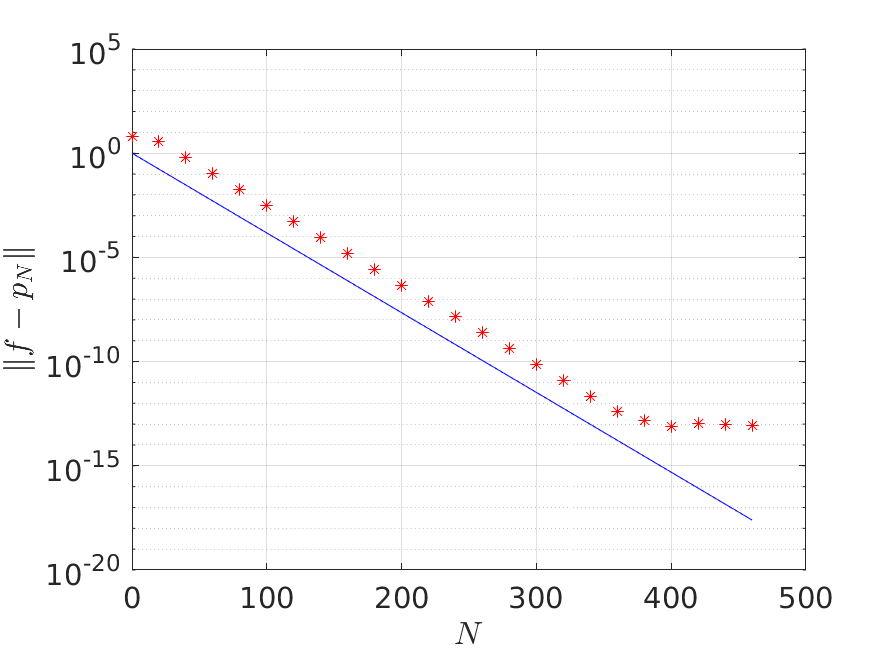
\includegraphics[scale=0.75]{tan(tan(x)).png}\caption{Convergence as $n\rightarrow\infty$ of the Chebyshev interpolant to $f(x)= \tan(\tan(x))$.}
\end{figure}

\item $f(x) = (1+x)\log(1+x)$. This function has a real singularity at $x=-1$. Hence, 
\begin{align*}
\rho = -1,
\end{align*}
and we have obtained the rate of convergence showed in the next figure.
\begin{figure}[H]
\centering
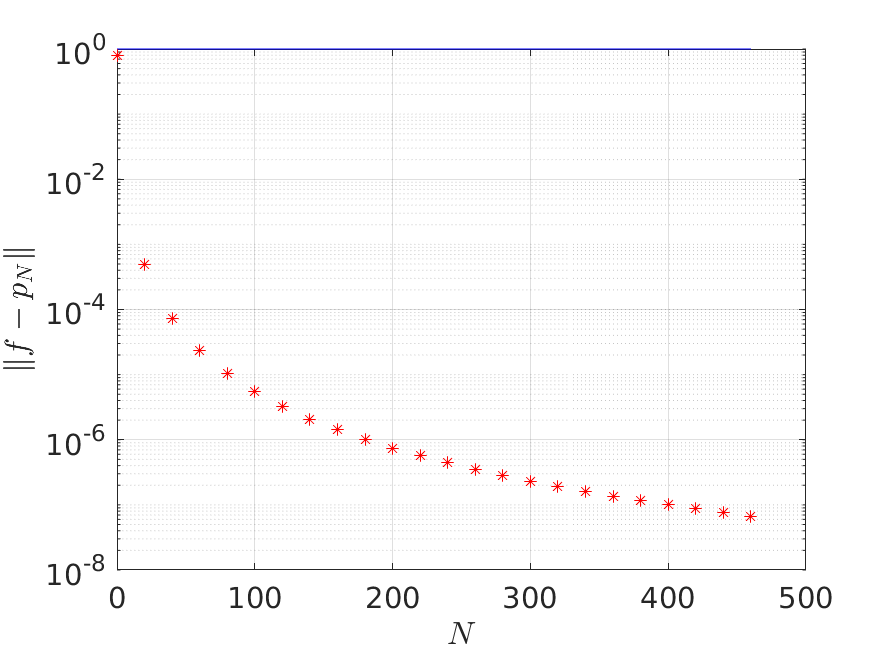
\includegraphics[scale=0.75]{(1+x)log(1+x)wrong.png}\caption{Convergence as $n\rightarrow\infty$ of the Chebyshev interpolant to $f(x)= (1+x)\log(1+x)$.}
\end{figure}
This figure is not right since the function does not satisfies the assumptions of \newline \textsc{Theorem 8.1}, it is not analytic in $[-1,1]$. The rate of convergence found is algebraic (much worse than the previous cases), as shown in the following figure.

\begin{figure}[H]
\centering
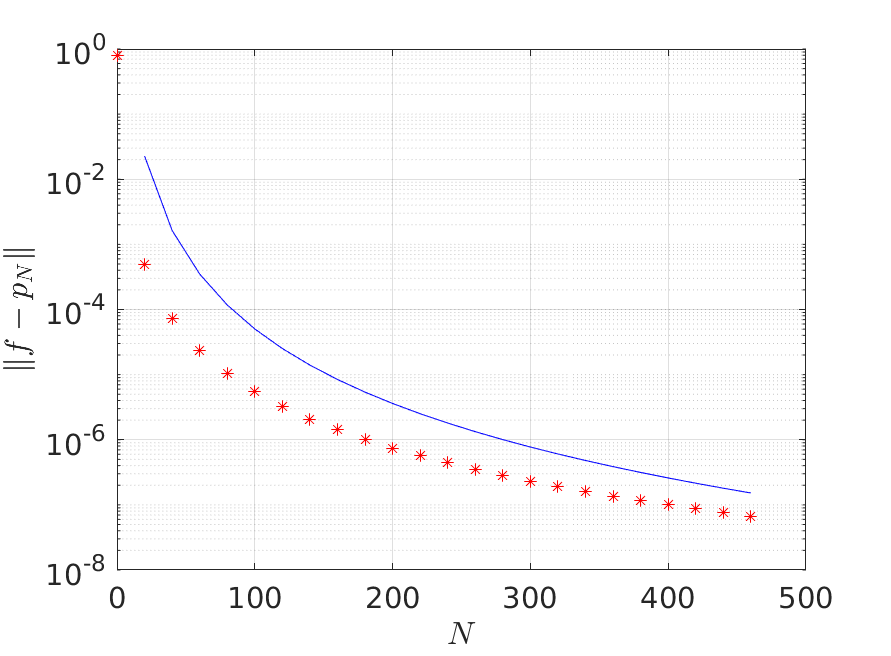
\includegraphics[scale=0.75]{(1+x)log(1+x)right.png}\caption{Algebraic convergence as $n\rightarrow\infty$ of the Chebyshev interpolant to \newline $f(x)= (1+x)\log(1+x)$.}
\end{figure}
\end{enumerate}

Overall, it has been tested that the larger the ellipse with foci $\{-1,1\}$ within which the function is analytic, the faster the convergence.
\subsection*{Matlab code for this problem}
\begin{verbatim}
rho = 0.5*pi+sqrt(0.25*pi^2-1);
orderAcuracy('tan(x)',50,2,rho)

rho = (0.5*pi+sqrt(0.25*pi^2+1));
orderAcuracy('tanh(x)',40,2,rho)

rho = (3+sqrt(8));
orderAcuracy('log((x+3)/4)/(x-1)',30,2,rho,'log1')

k = atan(pi/2);
rho = k+sqrt(k^2-1);
orderAcuracy('tan(tan(x))',460,20,rho)

rho = -1;
orderAcuracy('(1+x)*log(1+x)',460,20,rho,'(1+x)log(1+x)wrong')
orderAcuracy('(1+x)*log(1+x)',460,20,rho,'(1+x)log(1+x)right')

function orderAcuracy(func,Nmax,Nstep,rho,namefig)
    labelfontsize = 14;
    figformat = 'png';
    if nargin < 5
        namefig = func;
    end
    f = chebfun(func);
    nn = 0:Nstep:Nmax; ee = 0*nn;
    for j=1:length(nn)
        n = nn(j);
        fn = chebfun(f,n+1);
        ee(j) = norm(f-fn);
    end
    figure
    if strcmp(namefig,'(1+x)log(1+x)right')
        semilogy(nn,2000*nn.^(-3.8),'-b')
    else 
        semilogy(nn,rho.^(-nn),'-b')
    end
    hold on
    semilogy(nn,ee,'r*')
    grid on
    xlabel('$N$','interpreter','latex')
    ylabel('$\|f-p_N\|$','interpreter','latex')
    set(gca,'fontsize',labelfontsize)
    txt=['Latex/FIGURES\' namefig];
    saveas(gcf,txt,figformat)
end

% For the integral function
nn = 2:2:20;
err = 0*nn;
for k = 1:length(nn)
    N = nn(k);
    x = -.98:0.02:1;
    F = 0*x;
    FN = F;
    for j = 1:length(x) 
        f = chebfun('cos(t^2)', [-1 x(j)]);
        fN = chebfun('cos(t^2)', [-1 x(j)],N);
        F(j) = sum(f);
        FN(j) = sum(fN);
        F = [0 F]; FN = [0 FN]; x = [-1 x];
    end
    err(k) = norm(F-FN);
end
figure
semilogy(nn,err,'r*')
grid on
xlabel('$N$','interpreter','latex')
ylabel('$\|f-p_N\|$','interpreter','latex')
set(gca,'fontsize',labelfontsize)
txt='Latex/FIGURES\integral';
saveas(gcf,txt,figformat)
\end{verbatim}